\chapter{Investigating Developmental Disorders Diagnosis}
The target label of the data is modified to binary to examine the individual developmental disorders. After converting the label, each of the disorders are studied individually in this chapter. In the first section, ASD features and models are discovered, while in the second section, ADHD features and models are discovered. Finally, the last section VCFS features and models are built. Each of these sections help us understand these disorders and show results for children if these disorders existed exclusively in the children. This chapter discusses more specifically about their individual existence in the children. Also, impact of each of these individual parent-oriented reviews along with the IQ features on the developmental disorders will be discussed. Discussions are also done on the models that will we built for each of the developmental disorders using the features selected in chapter 3 by each of the feature selection algorithms.

\section{Austism Spectrum Disorder}
The target label diagnosis in the subgroup data has been modified to predict if a child has ASD or not. The data is modifies to understand and build models specific to ASD. This data will analyze ASD related features and models in greater depth. On this dataset different supervised learning techniques Logistic Regression, Decision Trees, K-Nearest Neighbors and Random Forest have been applied from the sklearn package in python and the following is the ROC curves obtained in figure \ref{fig:61}. The metrics for evaluation of these techniques are given in the table \ref{table:61}.
%table 6.1
\begin{table}[t]
\begin{center}
\begin{tabular}{|l|c|c|}
\hline
\textbf{ML Algorithm} & \textbf{Accuracy}&	\textbf{ROC Area}\\
\hline \hline
Random Forest&	98.64\%&	0.99137\\
\hline
Logistic Regression&	98.64\%&	0.96875\\
\hline
$K$- Nearest Neighbors($n$=3)&	85.135\%&	0.79202\\
\hline
Decision Tree&	97.297\%&	0.9375\\
\hline
\end{tabular}
\end{center}
\caption{ Supervised learning techniques comparison based on different metrics for ASD }
\label{table:61}
\end{table}

Among these supervised learning model, Random forest seems to be better fitting the `ASD data` when compared to other models. It has better Area Under Curve value than Logistic Regression model, even though the accuracy is same. By analyzing the results, it can be observed that tree based algorithms are doing a good job and the model for examining ASD can be repressed in the form of a tree. So, J48 algorithm is applied to describe the tree for our data, which can be seen in figure \ref{fig:62}.
\begin{figure}
\centering
  {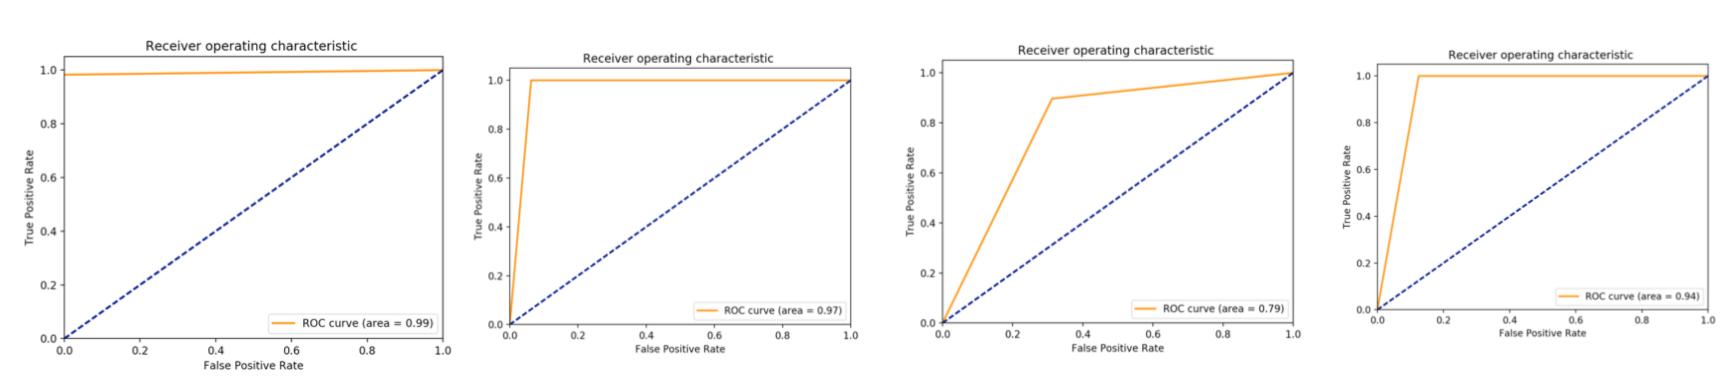
\includegraphics[width=0.8\textwidth]{Figures/Figure_6_1.png}}
  \caption{ ROC curve for ASD dataset \\a) Random Forest b) Logistic Regression c) KNN(n=3) d) Decision Tree }
  \label{fig:61}
\end{figure}
The accuracy of J48 algorithm is 96\% and ROC Area is 0.96. Also, for each individual group, the precision and recall are good. By combining the precision and recall, it can be seen that the F-measure for ASD subjects is 97\% and the F-measure for non-ASD subjects is 93\%. This shows that J48 is doing a good job at summarizing the results of the ASD data.


When training the Random Forest model, based on the features selected in chapter 3, table 6.2 shows the results of each of the feature selection algorithm. The features selected by ReliefF and RFE are performing better than the features selected by LASSO. The features selected by RFE is from the ADI parent-oriented review and hence, the ADI parent oriented review seems to be building better models when compared to the other parent oriented reviews.
\begin{figure}
\centering
{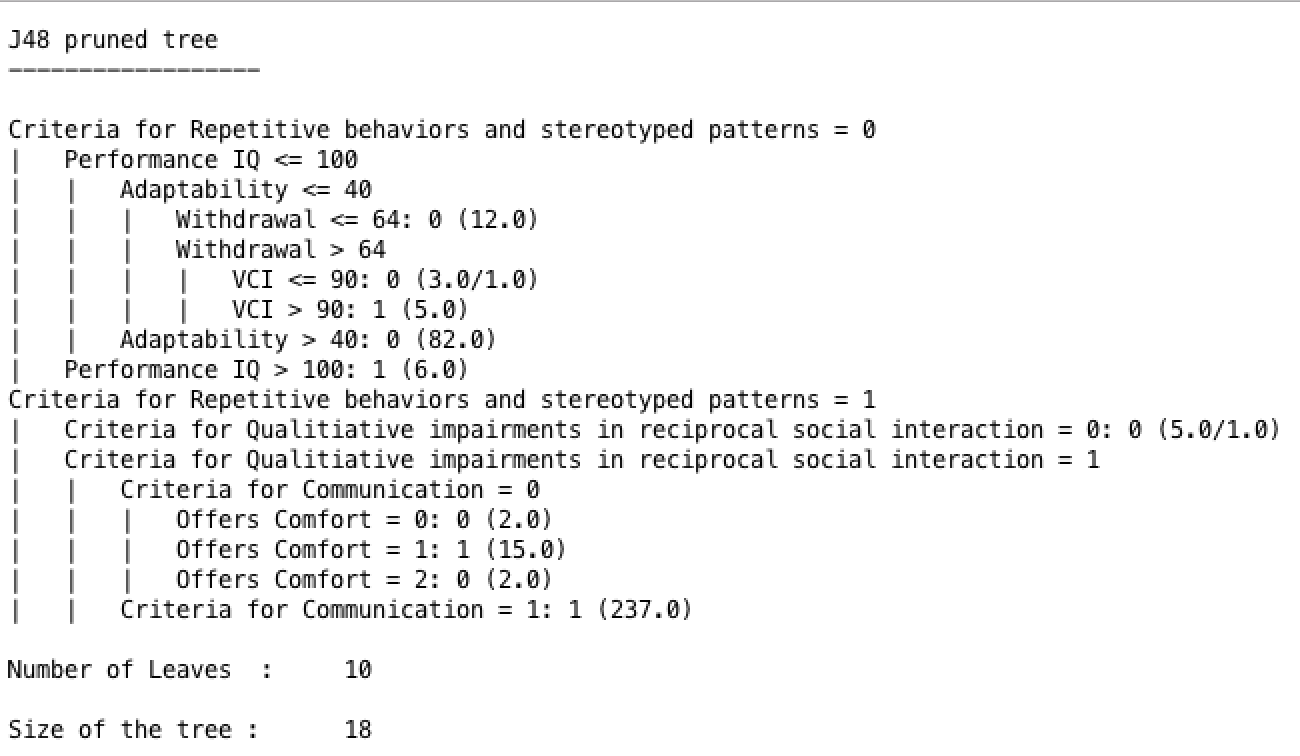
\includegraphics[width=0.6\textwidth]{Figures/Figure_6_2.png}}
  \caption{ J48 pruned tree for ASD  }
  \label{fig:62}
\end{figure}
%table 6.2
\begin{table}[h]
\begin{center}
\begin{tabular}{|l|c|c|c|}
\hline
\textbf{Feature Selection Algorithm}&	\textbf{Accuracy}&	\textbf{F-measure}&	\textbf{ROC Area}\\
\hline \hline
LASSO	&82.6 &	0.824	& 0.898\\
\hline
ReliefF &	91.3&	0.915&	0.967\\
\hline
RFE &	95.3 &	0.954 &	0.959\\
\hline
\end{tabular}
\end{center}
\caption{ Random Forest model trained with Feature Selection Algorithms for ASD }
\label{table:62}
\end{table}

\subsection{Predicting Diagnosis based on IQ feature set}
Based on the IQ features, different supervised learning techniques (random Forest, Naive Bayes, Logistic Regression) have been applied to predict ASD diagnosis for given dataset. These algorithms are used from WEKA by loading this data into it. The table \ref{table:63} shows the various metrics based on which the techniques are evaluated.
%table 6.3
\begin{table}[h]
\begin{center}
\begin{tabular}{|l|c|c|c|c|c|}
\hline
\textbf{ML Technique}&	\textbf{Precision}&	\textbf{Recall}&	\textbf{F-measure}&	\textbf{ROC Area}&	\textbf{Accuracy}\\
\hline \hline
Random Forest&	0.878&	0.878&	0.878&	0.930&	87.80\%\\
\hline
Naive Bayes&	0.693&	0.688&	0.691&	0.686&	68.83\%\\
\hline
Logistic Regression	&0.683&	0.713&	0.689&	0.796&	71.273\%\\
\hline
\end{tabular}
\end{center}
\caption{Supervised Learning Techniques applied on IQ features/variables for ASD }
\label{table:63}
\end{table}

Random Forest supervised learning technique is good at predicting ASD based on the IQ scores of the children with an accuracy of 87.8\%. The accuracy for model has dropped from 96\% as the features have been reduced to only IQ features. In comparison, it can be said that IQ features are not doing well compared to the entire feature set, so IQ feature set only is not a suitable method for predicting if a child has ASD or not.

\subsection{Predicting Diagnosis based on ADI feature set}
Further analysis has been done based on the ADI features, different supervised learning techniques have been applied to predict ASD diagnosis for given dataset. The table \ref{table:64} below shows the various metrics based on which the supervised learning techniques are evaluated.
%table 6.4
\begin{table}[h]
\begin{center}
\begin{tabular}{|l|c|c|c|c|c|}
\hline
\textbf{ML Technique}&	\textbf{Precision}&	\textbf{Recall}&	\textbf{F-measure}&	\textbf{ROC Area}&	\textbf{Accuracy}\\
\hline \hline
Random Forest&0.968&	0.967&	0.968&	0.991	&96.74\%\\
\hline
Naive Bayes&	0.948&	0.949&	0.948&	0.960&	94.85\%\\
\hline
Logistic Regression	&0.918&	0.916&	0.917	&0.954&	91.59\%\\
\hline
\end{tabular}
\end{center}
\caption{Supervised Learning Techniques applied on ADI feature set for ASD}
\label{table:64}
\end{table}

Random Forest supervised learning technique is good at predicting ASD based on the ADI feature/ variable scores of the children. Also, the ADI review is specifically designed for finding ASD behaviors in a child and hence, most models have high accuracy along with high ROC values. The accuracy of this model is similar to that of the J48 model and hence, ADI feature set could be used individually to diagnose a child with ASD.

\subsection{Predicting Diagnosis based on BASC feature set}
Based on the BASC feature set, different supervised learning techniques have been applied to predict ASD diagnosis for given dataset. The table \ref{table:65} shows the various metrics based on which the techniques are evaluated.
%table 6.5
\begin{table}[h]
\begin{center}
\begin{tabular}{|l|c|c|c|c|c|}
\hline
\textbf{ML Technique}&	\textbf{Precision}&	\textbf{Recall}&	\textbf{F-measure}&	\textbf{ROC Area}&	\textbf{Accuracy}\\
\hline \hline
Random Forest&0.920	&0.908&	0.910	&0.965&	90.78\%\\
\hline Naive Bayes&	0.915&	0.892&	0.895&	0.928&	89.15\%\\
\hline
Logistic Regression	&0.879	&0.875&	0.877	&0.936&	87.53\%\\
\hline
\end{tabular}
\end{center}
\caption{Supervised Learning Techniques applied on BASC feature set for ASD}
\label{table:65}
\end{table}

Random Forest supervised learning technique is good at predicting ASD based on the BASC feature scores of the children with an accuracy of 90.78\%. Even though the model accuracy has dropped to 91\% when compared to the J48 model, BASC features could still be used to predict if a child has ASD or not.

\subsection{Predicting Diagnosis based on VINE feature set}
Based on VINE feature set, different supervised learning techniques from WEKA have been applied to predict ASD diagnosis for given dataset. The table \ref{table:66} shows the various metrics based on which the techniques are evaluated. Random Forest and Logistic Regression supervised learning techniques are good at predicting ASD based on the VINE feature scores of the children with an accuracy of 88\%. However, the performance of both these models is less than 10\% when compared tot he J48 model and the model with ADI features. 
%table 6.6
\begin{table}[h]
\begin{center}
\begin{tabular}{|l|c|c|c|c|c|}
\hline
\textbf{ML Technique}&	\textbf{Precision}&	\textbf{Recall}&	\textbf{F-measure}&	\textbf{ROC Area}&	\textbf{Accuracy}\\
\hline \hline
Random Forest&0.884	&0.881&	0.882&	0.941&	88.07\%\\
\hline
Naive Bayes&0.792	&0.786	&0.788	&0.869&	78.59\%\\
\hline
Logistic Regression	&0.885&	0.883&	0.884&	0.917&	88.34\%\\
\hline
\end{tabular}
\end{center}
\caption{Supervised Learning Techniques applied on VINE feature set for ASD }
\label{table:66}
\end{table}

On the other hand, even though the model with VINE features is not doing well, it is better than the model with IQ features. So, only the VINE parent-oriented features cannot be used to diagnose a child with ASD.

\subsection{Observations}
When diagnosing a child with ASD, it can be seen that tree-based machine learning techniques like Random Forest and J48 are doing well. Also, it possible to diagnose a child with ASD using ADI and BASC parent-oriented review, but ADI parent-oriented review seems to be performing better than both the other parent oriented reviews. This could also be seen as the RFE feature selection algorithm in chapter 3, selects features from the ADI parent-oriented review and that is the best model from our feature selection models. The important features selected by the J48 model are a combination of all three parent-oriented reviews and are given below:
\begin{compactenum}
\item Offers Comfort
\item Criteria for Qualitative impairments in reciprocal social interaction
\item Criteria for Communication
\item Criteria for repetitive behaviors and stereotyped patterns
\item Adaptability
\item Withdrawal
\item Performance IQ 
\end{compactenum}

The features selected from the different feature selection algorithms in chapter 3 are compared to these features and 3 out of 7 of these features are same. It can be seen that J48 is converging the features selected by each of those algorithms. On an average, all the models to predict ASD have an accuracy of 90\%. The model with highest accuracy is with ADI parent-oriented review features. Therefore, it is observed that rather than using all the features in the data given, only the features of ADI parent-oriented reviews are sufficient, this supports the fact that ADI parent-oriented review is used to diagnose children with ASD.

\section{Attention Deficit/Hyperactivity Disorder}
The target label diagnosis in the subgroup data has been modified to predict if a child has ADHD or not. The dataset being used for this is converted, that is the class label is modified. On this dataset different supervised learning techniques Logistic Regression, Decision Trees, Naive Bayes and Random Forest have been applied and the following is the ROC curves obtained in figure \ref{figure:63}. The metrics for evolution of these techniques are given in the table \ref{table:67}.

%table 6.7
\begin{table}[h]
\begin{center}
\begin{tabular}{|l|c|c|}
\hline
\textbf{ML Algorithm }& \textbf{Accuracy}&	\textbf{ROC Area}\\
\hline \hline
Random Forest&	95.945\%&	0.90625\\
\hline
Logistic Regression&	77.027\%&	0.604525\\
\hline
$K$- Nearest Neighbors($n$=3)&	79.792\%	&0.8028\\
\hline
Decision Tree&	93.24\%&	0.8890\\
\hline
\end{tabular}
\end{center}
\caption{Supervised learning techniques based on different metrics for ADHD }
\label{table:67}
\end{table}

\begin{figure}
\centering
  {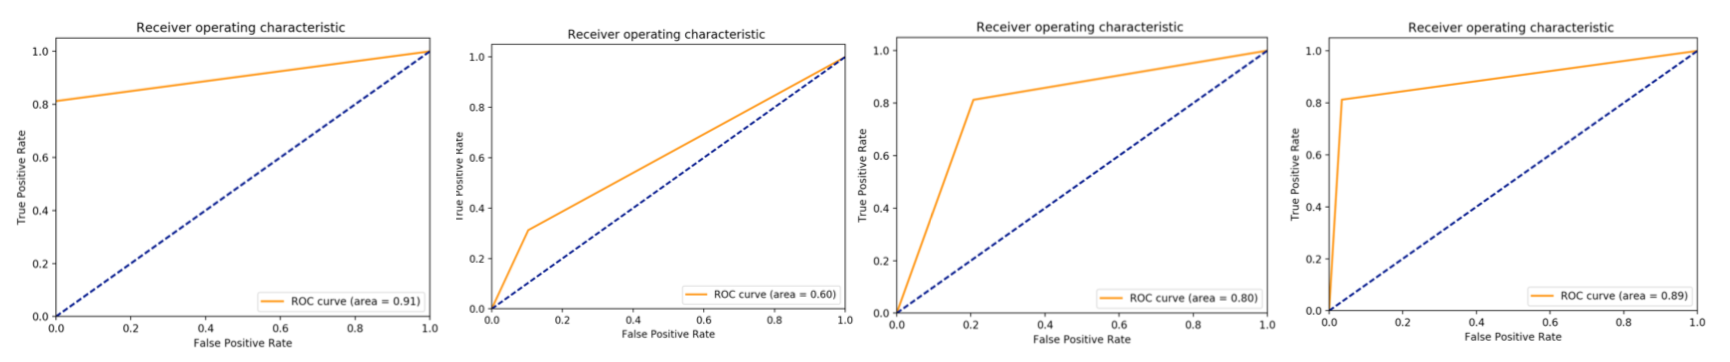
\includegraphics[width=0.8\textwidth]{Figures/Figure_6_3.png}}
  \caption{ ROC curve for ADHD dataset \\ a) Random Forest b) Decision Tree c) Naive Bayes d) Logistic Regression }
  \label{fig:63}
\end{figure}

Among these supervised learning models, Random Forest seems to be better fitting the `ADHD dataset` when compared to other models. It has better Area Under Curve value and accuracy. As the Random Forest is doing well for ADHD data, the features selected by each of the feature selection algorithm are trained using the random forest model and the performance of these three model is given in table \ref{table:68}.
%table 6.8
\begin{table}[h]
\begin{center}
\begin{tabular}{|l|c|c|c|}
\hline
\textbf{Feature Selection Algorithm}&	\textbf{Accuracy}&	\textbf{F-measure}&	\textbf{ROC Area}\\
\hline \hline
LASSO	&82.9\%&	0.813&	0.806\\
\hline
ReliefF &78.3\%	&0.764&	0.722\\
\hline
RFE &	95.9\%	&0.959&	0.942\\
\hline
\end{tabular}
\end{center}
\caption{ Random Forest model trained with Feature Selection Algorithms for ADHD}
\label{table:68}
\end{table}

When comparing the performance of models trained with the features from the three feature selection algorithms, it can be seen that RFE is doing better than the other two. Even though BASc is more commonly used to diagnose children with ADHD, this shows that ADI features can also do a good job at recognizing children with ADHD. 

As the random forest is doing well, another tree-based algorithm J48 is used to summarize our model and the prunes tree obtained from J48 algorithm is given in figure\ref{fig:64}. The algorithm had an accuracy of 94\% and it was good at diagnosing if children had ADHD or not. The F-measure for diagnosing ADHD is 83\% and without ADHD is 97\%. Since our data has small percentage of children when compared to those with ADHD, it can be seen that 83\% is comparable. Also, since the negative diagnosis percentage is high, it means that our model is doing well with trawl negative and can certainly till if a children doesn't have ADHD with good accuracy.
\begin{figure}
\centering
  {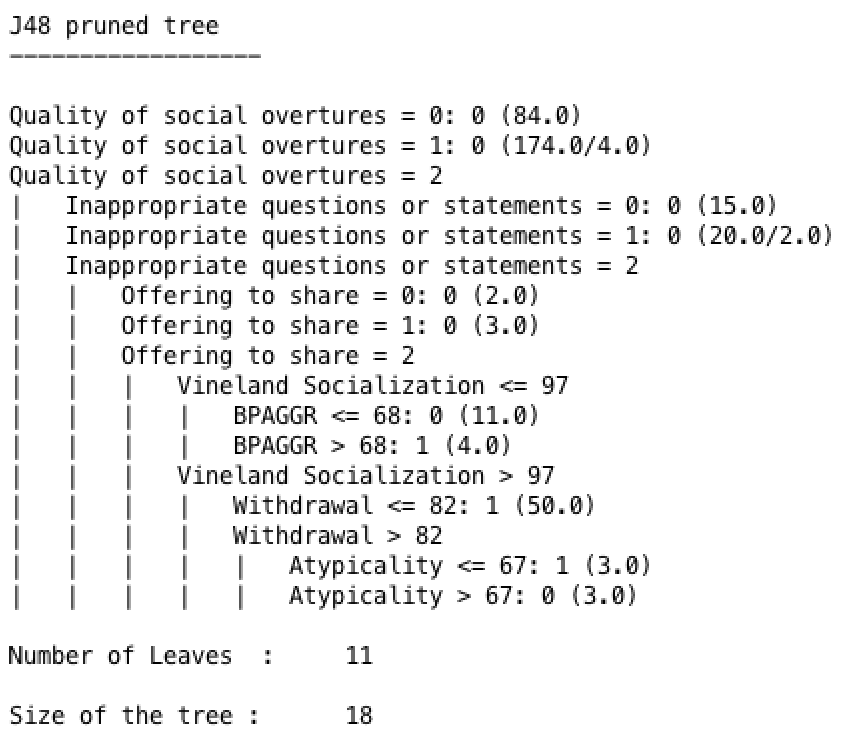
\includegraphics[width=0.6\textwidth]{Figures/Figure_6_4.png}}
  \caption{ J48 pruned tree for ADHD }
  \label{fig:64}
\end{figure}

\subsection{Predicting Diagnosis based on IQ feature set}
Based on the IQ feature set, different supervised learning techniques (Random Forest, Naive Bayes, Logistic Regression) have been applied to predict ADHD diagnosis for the modifies data. The table \ref{table:69} shows the various metrics based on which the techniques are evaluated.
%table 6.9
\begin{table}[h]
\begin{center}
\begin{tabular}{|l|c|c|c|c|c|}
\hline
\textbf{ML Technique}&	\textbf{Precision}&	\textbf{Recall}&	\textbf{F-measure}&	\textbf{ROC Area}&	\textbf{Accuracy}\\
\hline \hline
Random Forest&0.770&	0.799&	0.782&	0.714&	79.94\%\\
\hline
Naive Bayes&0.686	&0.818&	0.746	&0.556&	81.84\%\\
\hline
Logistic Regression	&0.792&	0.832&	0.772&	0.687&	83.19\%\\
\hline
\end{tabular}
\end{center}
\caption{Supervised Learning Techniques applied on IQ features/variables for ADHD  }
\label{table:69}
\end{table}

Logistic Regression supervised learning technique is good at predicting ADHD based on the IQ scores of the children. When comparing the performance of our model with the J48 model, it can be seen that the accuracy has dropped by 11\% and hence, only IQ features not sufficient at predicting if a child has ADHD.

\subsection{Predicting Diagnosis based on ADI feature set}
Now, further analysis is done based on the ADI feature set, different supervised learning techniques have been applied to predict ADHD diagnosis for modified data. The table \ref{table:610} shows the various metrics based on which the techniques are evaluated.
%table 6.10
\begin{table}[h]
\begin{center}
\begin{tabular}{|l|c|c|c|c|c|}
\hline
\textbf{ML Technique}&	\textbf{Precision}&	\textbf{Recall}&	\textbf{F-measure}&	\textbf{ROC Area}&	\textbf{Accuracy}\\
\hline \hline
Random Forest&0.981	&0.981	&0.981&	0.996	&98.10\%\\
\hline
Naive Bayes&0.934	&0.919&	0.923	&0.974	&91.86\%\\
\hline
Logistic Regression	&0.977&	0.976&	0.976&	0.687&	97.56\%\\
\hline
\end{tabular}
\end{center}
\caption{Supervised Learning Techniques applied on ADI features/variables for ADHD }
\label{table:610}
\end{table}

Random Forest supervised learning technique is good at predicting ADHD based on the ADI feature scores of the children and this also has high accuracy and ROC values for different classifier models. The Random Forest model with ADI feature set is better than the J48 model and Random Forest taking all the features into consideration. So, the J48 pruned tree using only the ADI features is given in figure 6.5. The accuracy of this model is 94.5\%, which is comparable to the previous J48 model. Also, the F-measure for diagnosing children with ADHD is 84.5\% which is more than our previous model diagnosis and for a children not having ADHD, the F-measure is 97\%. So, the ADI feature set is doing a better job at predicting if the child has ADHD better than the entire features of the data.
\begin{figure}
\centering
  {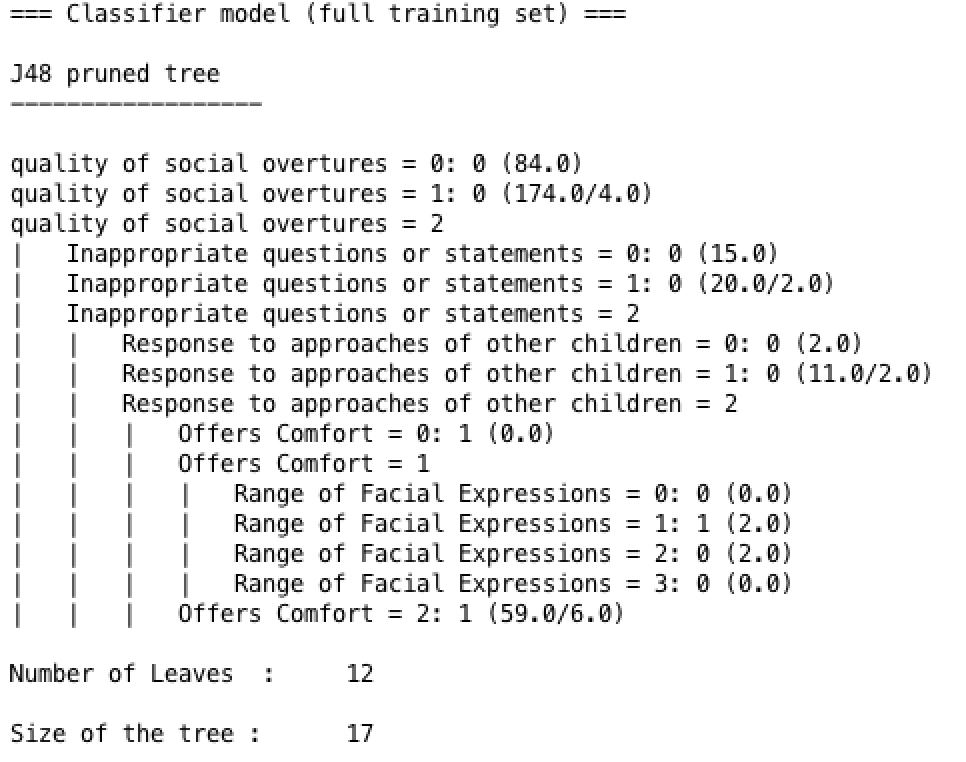
\includegraphics[width=0.8\textwidth]{Figures/Figure_6_5.png}}
  \caption{ J48 pruned tree for ADHD with ADI feature set}
  \label{fig:65}
\end{figure}

\subsection{Predicting Diagnosis based on BASC feature set}
Additional analysis is done using different supervised learning techniques to predict ADHD diagnosis for our converted data based on the BASC features/variables. The table \ref{table:611} shows the various metrics based on which the techniques are evaluated. Some of the supervised learning techniques applied from WEKA are Random Forest, Naive Bayes and Logistic Regression.
%table 6.11
\begin{table}[h]
\begin{center}
\begin{tabular}{|l|c|c|c|c|c|}
\hline
\textbf{ML Technique}&	\textbf{Precision}&	\textbf{Recall}&	\textbf{F-measure}&	\textbf{ROC Area}&	\textbf{Accuracy}\\
\hline \hline
Random Forest&0.794&	0.832&	0.793&	0.768&	83.19\%\\
\hline
Naive Bayes&0.792&	0.759&	0.773&	0.710&	75.88\%\\
\hline
Logistic Regression	&0.760&	0.802&	0.775&	0.709&	80.21\%\\
\hline
\end{tabular}
\end{center}
\caption{Supervised Learning Techniques applied on BASC features for ADHD }
\label{table:611}
\end{table}

Random Forest supervised learning technique is good at predicting ADHD based on the BASC scores of the children. However, when compared to the ADI model, our Random Forest classifier trains don BASC features has 10\% lower accuracy.

\subsection{Predicting Diagnosis based on VINE feature set}
Now, VINE features are applied to different supervised learning techniques to predict ADHD diagnosis for modifies data (target label modified to binary). The table \ref{table:612} shows the various metrics based on which the techniques are evaluated.

%table 6.12
\begin{table}[h]
\begin{center}
\begin{tabular}{|l|c|c|c|c|c|}
\hline
\textbf{ML Technique}&	\textbf{Precision}&	\textbf{Recall}&	\textbf{F-measure}&	\textbf{ROC Area}&	\textbf{Accuracy}\\
\hline \hline
Random Forest&0.685&	0.813&	0.744&	0.689&	81.30\%\\
\hline
Naive Bayes&0.851&	0.580&	0.627&	0.735	&57.9946\%\\
\hline
Logistic Regression	&0.687&	0.824&	0.749&	0.688&	82.38\%\\
\hline
\end{tabular}
\end{center}
\caption{Supervised Learning Techniques applied on VINE features for ADHD }
\label{table:612}
\end{table}

Logistic Regression supervised learning technique is good at predicting ADHD based on the VINE scores of the children. When the Logistic Regression model is compared to the ADI models, the performance of the model is not good, however, its performance is comparable to the model with BASC.
\subsection{Observations}
The analysis done in the above section shows that ADI parent-oriented review feature set is doing good at predicting if a child has ADHD. Moreover, our analysis shows that our models are good at eliminating true negatives that is there are better at diagnosing if the child doesn't have ADHD. The important ADI features, which can be used to diagnose a child with ADHD are given below:

\begin{compactenum}
\item Quality of social overtures
\item Inappropriate statements or questions
\item Group play with peers or friendships
\item Offers comfort
\item Response of approaches to other children
\item Range of facial expressions
\end{compactenum}

Most of these features selected were selected by our feature selection algorithms in chapter 3. Also, most of these features are important symptoms of diagnosing a child with ADHD.


\section{22Q Deletion Syndrome}
The target label diagnosis in the subgroup data has been modified into a binary attribute to predict if a child has ADHD or not. On this dataset different supervised learning techniques like Logistic Regression, Decision Trees, K-Nearest Neighbors and Random Forest have been applied and the following is the ROC curves obtained are present in figure\ref{fig:66}. These techniques have been applied from the sklearn package of python. The metrics for evaluation of these techniques are given in the table \ref{table:613}. 
%table 6.13
\begin{table}[h]
\begin{center}
\begin{tabular}{|l|c|c|}
\hline
\textbf{ML Algorithm} & \textbf{Accuracy}&	\textbf{ROC Area}\\
\hline \hline
Random Forest&	98.648\%&	0.99107\\
\hline
Logistic Regression&	97.297\%&	0.98214\\
\hline
$K$- Nearest Neighbors($n$=3)&91.891\%	&0.88988\\
\hline
Decision Tree&	83.7837\%&	0.79861\\
\hline
\end{tabular}
\end{center}
\caption{Supervised learning techniques based on different metrics for VCFS }
\label{table:613}
\end{table}

Among these supervised learning models, Random Forest seems to be better fitting the `VCFS dataset` when compared to other models, it has better Area Under Curve value and accuracy. Even Logistic Regression algorithm is fitting the data well and has a good accuracy of 97\%. Using the J48 algorithm, the pruned tree in figure \ref{fig:67} is a summarization of the model.
\begin{figure}
\centering
  {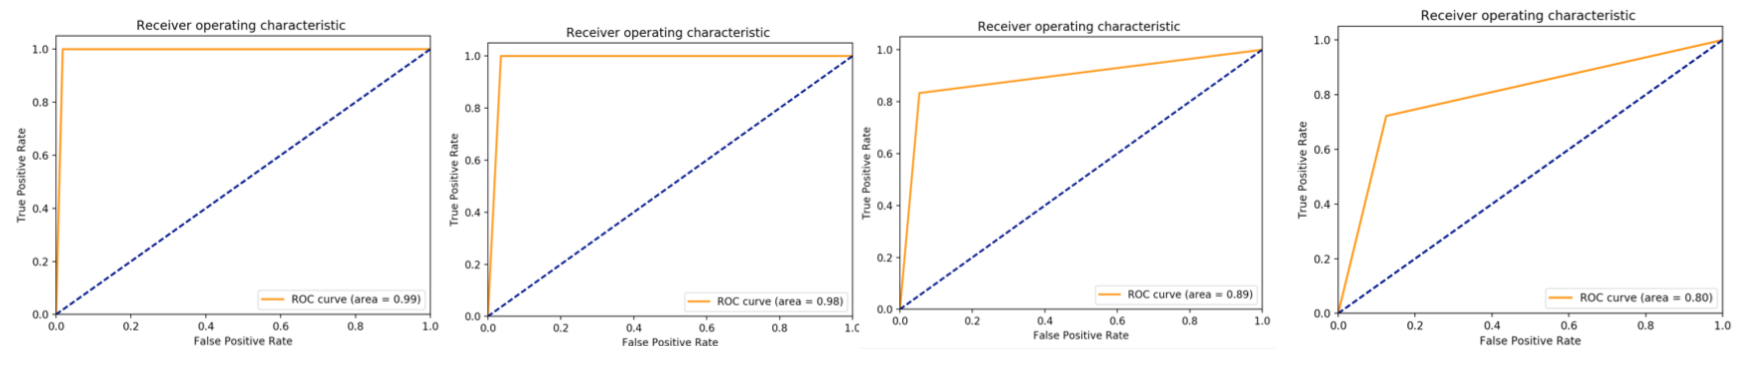
\includegraphics[width=0.8\textwidth]{Figures/Figure_6_6.png}}
  \caption{ ROC curve for VCFS dataset \\ a) Random Forest b) Decision Tree c) Naive Bayes d) Logistic Regression }
  \label{fig:63}
\end{figure}
\begin{figure}
\centering
  {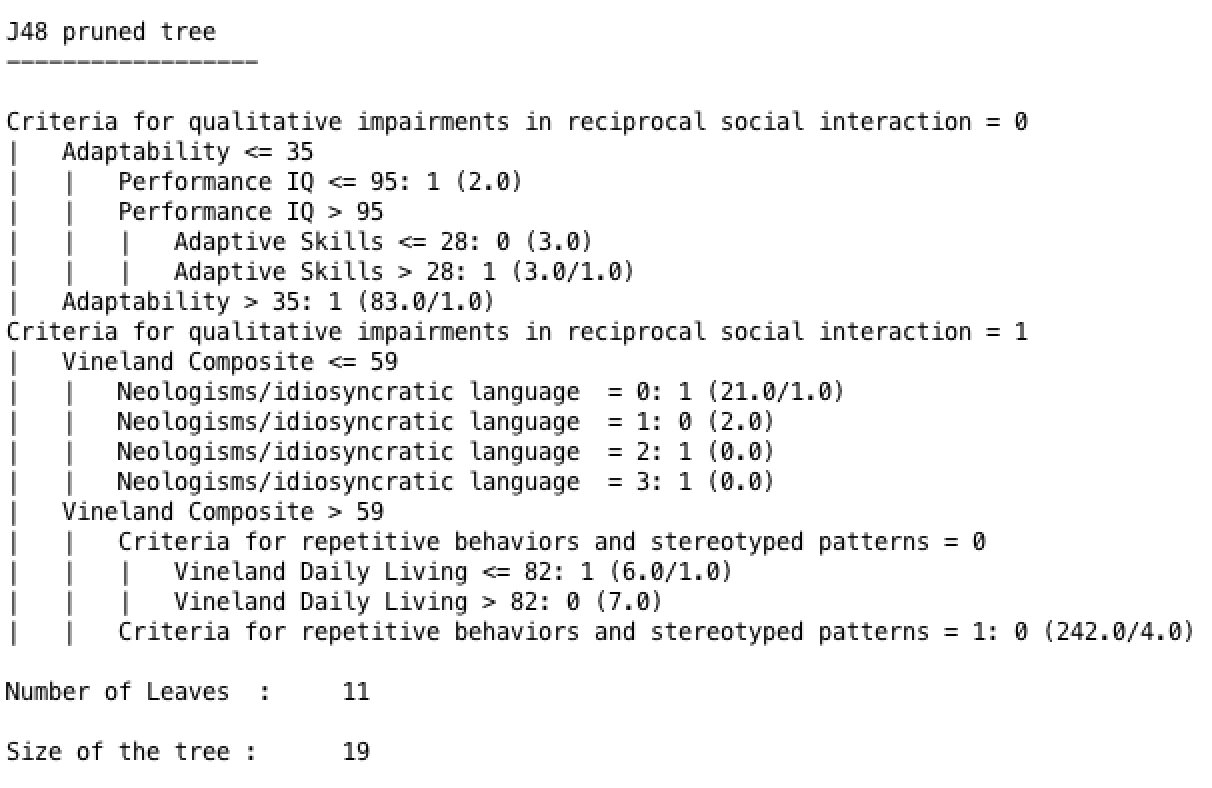
\includegraphics[width=0.8\textwidth]{Figures/Figure_6_7.png}}
  \caption{ J48 pruned tree for VCFS}
  \label{fig:67}
\end{figure}
The accuracy of this J48 is 93.4\%. The F-measure of diagnosing the children with VCFS is 90\% and the F-measure of not diagnosing the child with VCFS is 95.3\%. The performance of this model is not has good as the Random Forest model or Logistic Regression model, but it is comparable and a good way of representing our data. Now, the features selected in chapter 3 are used to train the Random Forest model as it is performing the best with our data and the results of the models for each feature selection algorithm are given in table \ref{table:614}. Among all the feature selection algorithms, LASSO is performing the best.
%table 6.14
\begin{table}[h]
\begin{center}
\begin{tabular}{|l|c|c|c|}
\hline
\textbf{Feature Selection Algorithm}&	\textbf{Accuracy}&	\textbf{F-measure}&	\textbf{ROC Area}\\
\hline \hline
LASSO	&92.4\%&	0.924&	0.974\\
\hline
ReliefF &787.2\%&	0.873&	0.922\\
\hline
RFE &	90.2\%	&0.903&	0.951\\
\hline
\end{tabular}
\end{center}
\caption{ Random Forest model trained with Feature Selection Algorithms for VCFS}
\label{table:614}
\end{table}

\subsection{Predicting Diagnosis based on IQ feature set}
Based on the IQ feature set, different supervised learning techniques have been applied to predict VCFS diagnosis for given dataset. The table \ref{table:615} shows the various metrics based on which the techniques are evaluated.
%table 6.15
\begin{table}[h]
\begin{center}
\begin{tabular}{|l|c|c|c|c|c|}
\hline
\textbf{ML Technique}&	\textbf{Precision}&	\textbf{Recall}&	\textbf{F-measure}&	\textbf{ROC Area}&	\textbf{Accuracy}\\
\hline \hline
Random Forest&0.883&	0.883&	0.883&	0.948&	88.34\%\\
\hline
Naive Bayes&0.692&	0.694&	0.693&	0.712&	69.37\%\\
\hline
Logistic Regression	&0.747&	0.759&	0.746&	0.825&	75.88\%\\
\hline
\end{tabular}
\end{center}
\caption{Supervised Learning Techniques applied on IQ features/variables for VCFS}
\label{table:615}
\end{table}

Out of all the supervised learning techniques, Random Forest is the best at predicting VCFS for children. However, compared to the previous Random Forest and J48 model, the accuracy has dropped by 7\% and hence, predicting ADHD with only the IQ feature set is not a good idea.

\subsection{Predicting Diagnosis based on ADI feature set}
Based on the ADI review feature set, different supervised learning techniques have been applied to predict VCFS diagnosis for given dataset. The table \ref{table:616} shows the various metrics based on which the techniques are evaluated.
%table 6.16
\begin{table}[h]
\begin{center}
\begin{tabular}{|l|c|c|c|c|c|}
\hline
\textbf{ML Technique}&	\textbf{Precision}&	\textbf{Recall}&	\textbf{F-measure}&	\textbf{ROC Area}&	\textbf{Accuracy}\\
\hline \hline
Random Forest&0.943&	0.943&	0.942&	0.981&	94.30\%\\
\hline
Naive Bayes&0.913&	0.913&	0.913&	0.927&	91.32\%\\
\hline
Logistic Regression& 0.922&	0.921&	0.922&	0.943&	92.14\%\\
\hline
\end{tabular}
\end{center}
\caption{Supervised Learning Techniques applied on ADI feature set for VCFS}
\label{table:616}
\end{table}

ADI feature set is doing better than IQ feature set when diagnosing children with VCFS. The best learning technique is Random Forest, but the performance of this model is low when compared to the Random Forest model with the entire dataset. However, ADI parent-oriented review features could be used to predict if a child has VCFS.

\subsection{Predicting Diagnosis based on BASC feature set}
Based on the BASC review feature set, different supervised learning techniques(Random Forest, Logistic Regression, Naive Bayes) have been applied to predict VCFS diagnosis for given dataset. The table \ref{table:617} shows the various metrics based on which the techniques are evaluated. 
%table 6.17
\begin{table}[h]
\begin{center}
\begin{tabular}{|l|c|c|c|c|c|}
\hline
\textbf{ML Technique}&	\textbf{Precision}&	\textbf{Recall}&	\textbf{F-measure}&	\textbf{ROC Area}&	\textbf{Accuracy}\\
\hline \hline
Random Forest&0.956&	0.951&	0.952&	0.983&	95.12\%\\
\hline
Naive Bayes&0.927&	0.916&	0.918&	0.933&	91.59\%\\
\hline
Logistic Regression& 0.896&	0.894&	0.895&	0.954&	89.43\%\\
\hline
\end{tabular}
\end{center}
\caption{Supervised Learning Techniques applied on BASC feature set for VCFS}
\label{table:617}
\end{table}

Among the different supervised learning techniques for predicting VCFS, Random Forest supervised learning technique is good to predict based on the BASC feature/variable scores of the children with accuracy of 95\%. So, the BASC parent oriented review is better than the ADI parent oriented review for predicting VCFS.

\subsection{Predicting Diagnosis based on VINE feature set}
Based on the VINE review feature set, different supervised learning techniques{random Forest, Naive Bayes, Logistic Regression} have been applied to predict VCFS diagnosis for given dataset. These supervised learning techniques are applied from WEKA. The table \ref{table:618} shows the various metrics based on which the techniques are evaluated. 
%table 6.18
\begin{table}[h]
\begin{center}
\begin{tabular}{|l|c|c|c|c|c|}
\hline
\textbf{ML Technique}&	\textbf{Precision}&	\textbf{Recall}&	\textbf{F-measure}&	\textbf{ROC Area}&	\textbf{Accuracy}\\
\hline \hline
Random Forest&0.887&	0.886&	0.887&	0.961&	88.16\%\\
\hline
Naive Bayes&0.812&	0.808&	0.809&	0.897&	80.75\%\\
\hline
Logistic Regression&0.891&	0.892&	0.891&	0.928&	89.15\%\\
\hline
\end{tabular}
\end{center}
\caption{Supervised Learning Techniques applied on VINE feature set for VCFS}
\label{table:618}
\end{table}

Even in this case for predicting VCFS, Random Forest supervised learning technique is good to predict based on the VINE feature scores of the children with accuracy of 88\% as it has a better ROC value when compared with Logistic Regression which has an accuracy of 89\%. The performance of this model is comparable to the performance of the IQ feature set models, but its performance is lower than all other models. As the children who have taken VINE is only 47\%, the model performance is good in comparison and it could be more generalized than other models.

\subsection{Observations}
Tree-based machine learning algorithms particularly Random Forest algorithm is doing best for diagnosing children with VCFS. Among the four different feature sets, BASC parent oriented reviews are doing the best. Even the though the performance of BASC parent-oriented review is good and comparable, the model with the entire features is out performing all the other models. The best features in the pruned tree are a combination of all the four feature sets present in our data.  Also, the best features selected by the J48 algorithm are as follows:
\begin{compactenum}
\item Adaptability
\item Criteria for Qualitative impairments in reciprocal social interaction
\item Performance IQ
\item Adaptive skills
\item Vineland Composite
\item Neologisms/idiosyncratic language
\item Criteria for Repetitive behaviors and stereotyped patterns
\item Vineland Daily Living
\end{compactenum}
Out of the 8 features selected by J48 algorithm, 6 of them were selected by our feature selection algorithms. Hence, these features are important for diagnosing a child with VCFS and no individual feature set out of the four feature sets could be used to diagnose children with VCFS. However, these features have more importance over other features in the given data and a model trained with these features performs well for predicting VCFS in children.